\chapter{基于隐式表示的薄壳结构雕刻设计}

\section{引言}
薄壳结构以其纤薄和弯曲的形状承载载荷,这种结构特别优雅和高效。它们在我们的生活环境中以各种尺寸广泛存在,在满足力学性能的同时提供了艺术美感的视觉体验~\cite{adriaenssens2014,melaragno2012}。近年来,基于壳体结构的曲面设计受到艺术家和研究人员的广泛关注~\cite{Pietroni2015, Chen2016, Liu2020}。其中,雕刻是设计壳体结构的一种流行方式~\cite{Yang2019,stadlbauer2020}。经过精巧的雕刻设计,壳体结构可以具有更高的艺术感,并在医疗和轻量化应用中得到广泛实践~\cite{Zhang2017,Rao2019}。

现代计算机图形学技术的发展已经引领了壳体结构雕刻设计方法的日益多样化,例如基于纹理合成的方法~\cite{Dumas2015},基于镶嵌的方法~\cite{Pietroni2015}和基于重复模板的方法~\cite{schumacher2016}。作为一种材料减少过程,雕刻设计的核心问题是在设计过程中维持壳体结构的力学性能和功能。现有的大多数方法都侧重于显式表示,如多边形网格等,这不利于结构分析和参数优化。
由于雕刻壳体结构的拓扑和几何结构高度复杂,采用传统有限元方法(FEM)~\cite{bucalem1997,cirak2002} 进行力学响应分析非常耗时。此外,在现有的设计技术中,设计、分析和优化通常是分离的,在不同阶段经常需要重复重新划分网格~\cite{panetta2019}。由于缺乏统一的表示方法和有效的优化技术,在壳体结构上进行雕刻设计并非易事。

本文研究提出了一种隐式参数化方法来设计轻量级薄壳结构,并通过参数优化保证结构的物理可靠性,如图~\ref{fig:thin-shell-1} 所示。具体地,通过在输入薄壳结构上分布重复模板图案并对其进行雕刻来完成设计,用隐式表示的薄壳结构的模板图案可以直接用函数进行设计、分析和优化,本文通过优化模板图案的尺寸和方向等属性,在雕刻设计的同时最大化壳体结构的刚度。与基于传统有限元的网格方法相比,本文方法由于避免了显式模型的生成和分析过程中的重新网格剖分,在保证足够精度的前提下大大提高了计算效率。此外,本文还通过对图案模板的不同函数操作,实现了对偶雕刻设计,进一步增强了薄壳结构设计的丰富性。本文通过在多种薄壳结构模型上的测试,并实施了仿真和对比试验来证明该方法的有效性和高效性。

\begin{figure}[!b]
    \centering
    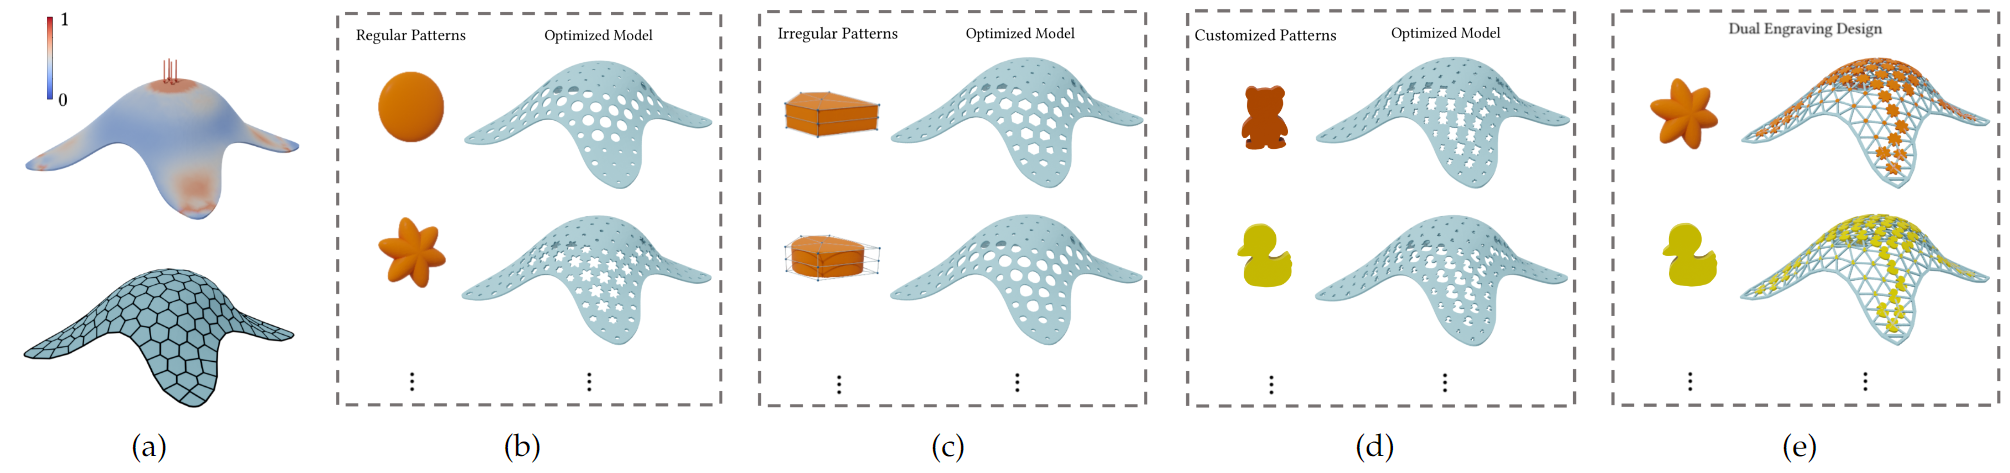
\includegraphics[width=1.0\linewidth]{./figures/thin-shell-1}
    \caption{基于隐式表示的                              薄壳(对偶)雕刻设计优化方法}
    \label{fig:thin-shell-1}
\end{figure}

\section{研究方法}

本方法基于结构的隐式表示设计了一种用于薄壳结构雕刻设计的参数化方法,算法流程如图~\ref{fig:thin-shell-pipeline} 所示。首先,使用函数表示构建三种类型的图案模板,包括规则图案、不规则图案和用户指定的个性化图案。这些图案模板具有可调整的属性, 例如位置、方向和大小, 可以通过参数控制(第~\ref{subsec:parametric-design}节)。然后,将这些模板图案用于壳体结构的雕刻。由于使用有向距离场(SDF)表示输入壳体,因此可以在图案模板和壳体模型之间执行函数布尔运算。最后,为了确保雕刻壳体结构的完整性,引入了结构力学问题的优化模型。以最小应变能为目标,给定体积为约束,该框架可以根据结构响应分析优化图案的属性变量。优化后的(对偶)雕刻壳体结构可以简单地用函数的零等值面表示(第~\ref{}节)。在各种壳体模型上成功实现了该算法,并进行了多组实验,验证了该框架的有效性和鲁棒性(第~\ref{}节)。


\begin{figure}[htbp]
    \centering
    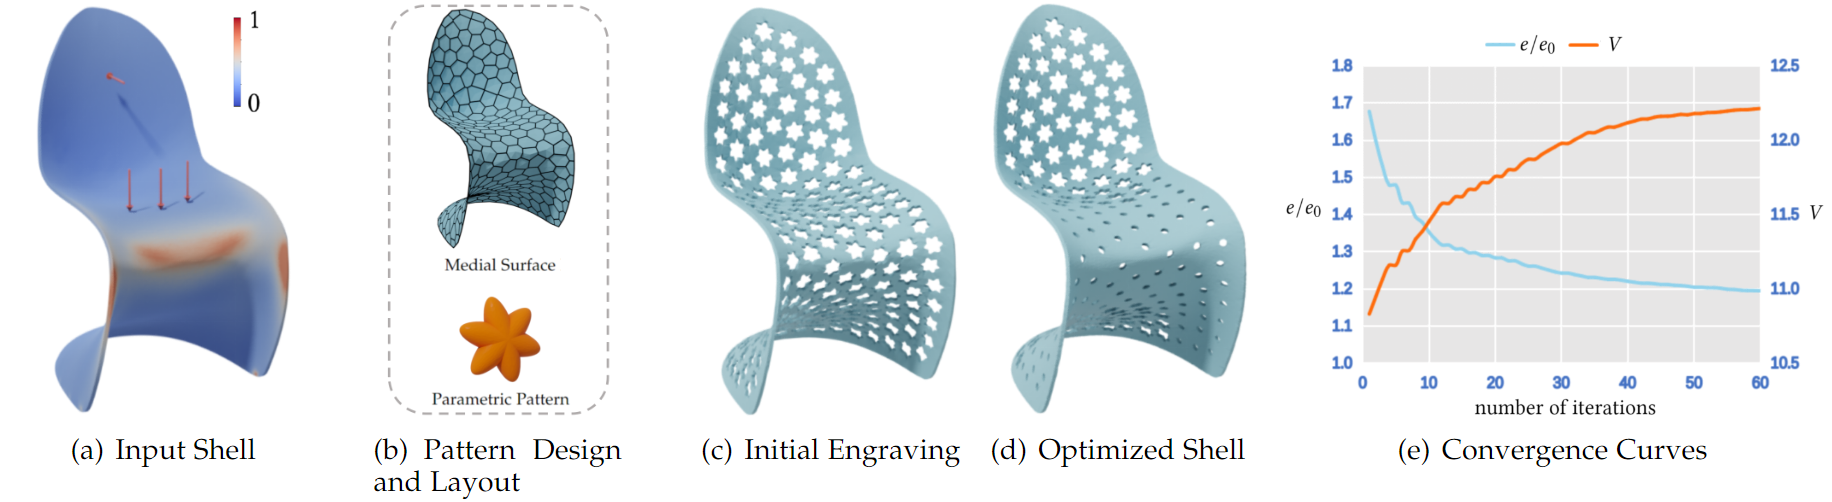
\includegraphics[width=1.0\linewidth]{./figures/thin-shell-pipeline}
    \caption{薄壳雕刻设计方法流程图}
    \label{fig:thin-shell-pipeline}
\end{figure}


\subsection{参数化设计}
\label{subsec:parametric-design}
本文算法采用隐式函数来表示输入模型和图案模板,从而将复杂的结构优化转化为可控参数设计问题,如此便可以高效、鲁棒和可扩展的方式进行结构的设计和优化。

\subsubsection{图案模板设计}
本文提出了三种用于薄壳结构雕刻设计的图案模板类型,包括规则图案、非规则图案和个性化图案,所有这些图案都可以用隐式函数表示。

\paragraph{规则图案模板。}首先考虑旋转对称的规则图案,并使用超椭球方程构造它们,
\begin{equation}
    \label{eq-ellipsoid}
    E(\mathbf{r})=\left(\frac{\hat{x}}{L_1}\right)^p+\left(\frac{\hat{y}}{L_2}\right)^p+\left(\frac{\hat{z}}{L_3}\right)^p-1,
\end{equation}
其中 $\mathbf{r}=(x, y, z)^\top\in\Omega$ 为三维空间 $\mathbb{R}^3$ 中的设计域,  $\mathbf{c}_0=(x_0,y_0,z_0)^\top$ 是超椭球的中心坐标。
定义 $\hat{\mathbf{r}}=(\hat{x}, \hat{y}, \hat{z})^\top=\mathbf{R}(\mathbf{r}-\mathbf{c}_0)$, 其中 $\mathbf{R}=\{R_{ij}\}_{3\times 3}$ 为旋转矩阵用于调整超椭球的方向。 $L_1$,$L_2$,和 $L_3$ 是超椭球的三个轴长,$p$ 是形状因子,是一个大于零的偶数。当 $p$ 增大时,超椭球逼近一个长方体。

通过控制少量参数,多个超椭球可以构成丰富复杂的图案结构。可以在局部坐标系中围绕其中心点旋转一个超椭球,以获得新的图案, 如图~\ref{fig-ellip} 所示。具体地,假设一个规则图案模板是由 $n$ 个超椭球$\{E_i\}_{i=1}^n$ 组成,第$k$个超椭球的旋转角度为 $\frac{k\pi}{n}$,$k=1,2,\cdots,n$。因此,可通过旋转矩阵 $\Lambda(\frac{k\pi}{n})\mathbf{R}$ 计算超椭球 $E_k$ 的方向,其中 $\Lambda(\theta)$ 是绕 $z$ 轴旋转矩阵:
\begin{equation}
    \Lambda(\theta)=
    \begin{pmatrix}
        \cos\theta & \sin\theta & 0 \\
        -\sin\theta & \cos\theta  & 0 \\
        0                  & 0                   & 1
    \end{pmatrix}.
\end{equation}
最终,规则图案模板就表示为这些超椭球 $\{E_i\}_{i=1}^n$ 的布尔并,即函数形式:
\begin{equation}
    P(\mathbf{r})=\min(E_1, E_2, \cdots, E_n).
\end{equation}
总的来说,一个规则图案模板具有可设计变量 $\{\mathbf{c}_0, L_1, L_2, L_3, \mathbf{R}, n, p\}$,可以根据应用需求优化这些参数来控制雕刻壳体结构的艺术和物理属性。
\begin{figure}[htbp]
    \centering
    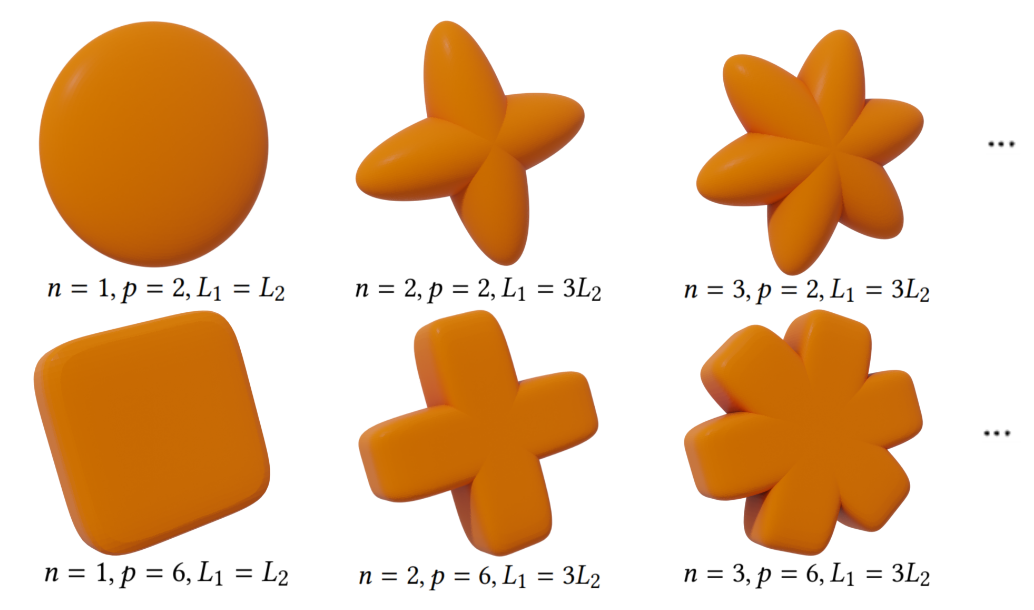
\includegraphics[width=0.8\linewidth]{./figures/multi-ellips}
    \caption{规则图案模板示例}
    \label{fig-ellip}
\end{figure}

\paragraph{非规则图案模板。}
非规则图案具有自由的轮廓,本文用连续函数表示这些图案。具体地,采用被广泛使用的 Voronoi 结构图案,将 Voronoi 图的顶点设置为初始控制点,利用 B-样条来表示非规则图案。
如图~\ref{fig-irregular}所示, 给定一个 Voronoi 单元,其顶点为 $\{\mathbf{p}^0_i\}_{i=1}^m$,质心为 $\mathbf{c}_0=(x_0,y_0,z_0)^\top$,外法向量为 $\mathbf{n}$,则可以设置新的图案控制点为
\begin{equation}
	\mathbf{p}_i=s\mathbf{p}^0_i+(1-s)\mathbf{c}_0,
\end{equation}
其中 $0<s<1$ 是一个偏移因子。
\begin{figure}[htbp]
    \centering
    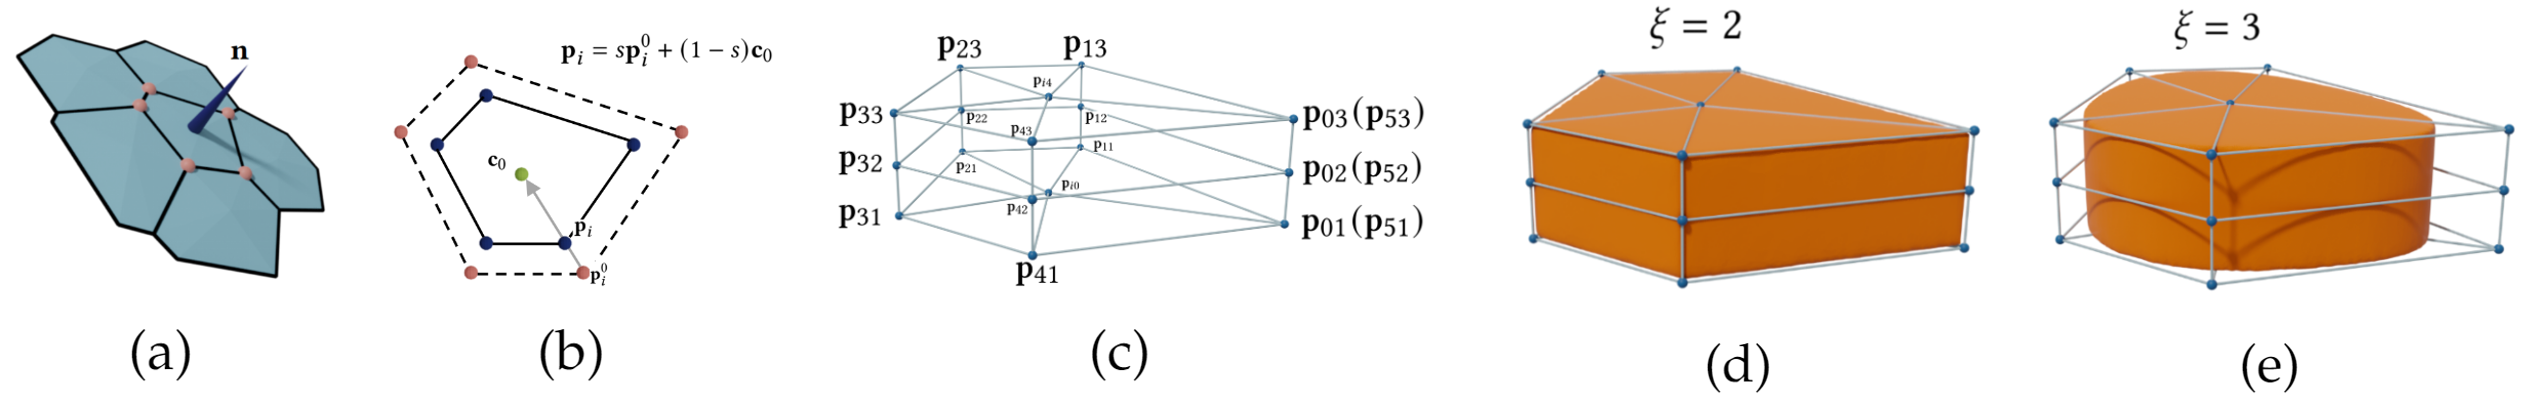
\includegraphics[width=1.0\linewidth]{./figures/iregular-pattern}
    \caption{基于Voronoi结构的非规则图案模板构造示意图}
    \label{fig-irregular}
\end{figure}
为了使用B样条构造一个封闭的模板曲面,设计控制网格如下(见图~\ref{fig-irregular}(c)):
\begin{equation}
	\begin{split}
	&\mathbf{p}_{i0}=\mathbf{c}_0-\frac{h_0}{2}\mathbf{n},\,\,i=0,1,\cdots,m,\\
	&\mathbf{p}_{i1}=\mathbf{p}_i-\frac{h_0}{2}\mathbf{n},\,\,i=1,\cdots,m,\,\,\mathbf{p}_{01}=\mathbf{p}_{m1}, \\
	&\mathbf{p}_{i2}=\mathbf{p}_i,\,\,i=1,\cdots,m,\,\,\mathbf{p}_{02}=\mathbf{p}_{m2}, \\	
	&\mathbf{p}_{i3}=\mathbf{p}_i+\frac{h_0}{2}\mathbf{n},\,\,i=1,\cdots,m,\,\,\mathbf{p}_{03}=\mathbf{p}_{m3}, \\
	&\mathbf{p}_{i4}=\mathbf{c}_0+\frac{h_0}{2}\mathbf{n},\,\,i=0,1,\cdots,m,
	\end{split}
\end{equation}
其中 $h_0$ 是输入薄壳结构的厚度。然后,一个非规则图案模板就可以隐式表示为:
\begin{equation}
	P(\mathbf{r})=||\mathbf{r}-\mathbf{c}_0||-d(u,v)=0,
\end{equation}
其中 $d(u,v)$ 是距离函数,可以按如下插值形式:
 \begin{equation}
 	d(u,v)=\left\|\sum_{i=0}^m\sum_{j=0}^4N_{i,\xi}(u)N_{j,\eta}(v)\mathbf{p}_{ij}-\mathbf{c}_0\right\|,
 \end{equation}
其中 $\|\cdot\|$ 是$\mathbb{R}^3$上的欧几里得范数,$N_{i,\xi}(u)$ 和 $N_{j,\eta}(v)$ 是带有曲面参数 $u$ 和 $v$ 的B样条基函数~\cite{cohen2001}。方法中设置 $u\in[-\pi, \pi]$,$v\in[0, \pi]$ 并采用均匀间隔的结点。$\xi$ 和 $\eta$ 是B样条基函数的阶数。在实验中,$\eta=2$,$\xi$ 用于控制非规则图案的光滑度。对于非规则图案,可控制的设计变量是 $\{\mathbf{c}_0, s,\xi\}$。

\paragraph{个性化图案模板。}
个性化图案模板具有用户可自定义的轮廓,它们应该是一个薄片平面模型,其厚度与输入壳结构的厚度有关。为了以标准化的方式构建定制图案,本文计算了包围图案二维轮廓的最小圆~\cite{Sven1991},并通过圆的半径限制图案的尺寸。以最小圆的圆心为局部坐标系的中心,通过沿$z$轴偏移平面模型,可以获得厚度为 $h_0$ 的个性化图案。为了统一函数表示,本文使用径向基函数拟合定制图案。类似地,本文应用缩放因子 $\mathbf{s}=(s_x,s_y,s_z)^\top$ 和旋转矩阵 $\mathbf{R}$ 来控制图案的大小和方向。最后,将定制图案表示为拟合函数的零等值面
\begin{equation}	
    P(\mathbf{r})=\sum_{i=1}^m\omega_i\varphi(\|\hat{\mathbf{r}}-\mathbf{r}_i\|)+Q(\hat{\mathbf{r}})=0,
\end{equation}
其中 $\hat{\mathbf{r}}=\mathbf{s}^\top\mathbf{R}(\mathbf{r}-\mathbf{c}_0)$, $\mathbf{c}_0=(x_0, y_0, z_0)$ 是模板的中心坐标, $\{\mathbf{r}_i\}_{i=1}^m$ 是图案模板所占空间钟均匀采样得到的点(默认$m=1000$),$\varphi(t)=t^2\log(t)$是薄板样条基函数,$Q(\mathbf{r})=\omega_{m+1}x+\omega_{m+2}y+\omega_{m+3}z+\omega_{m+4}$, $\{\omega_i\}_{i=1}^{m+4}$ 是拟合系数。
\begin{figure}
    \centering
    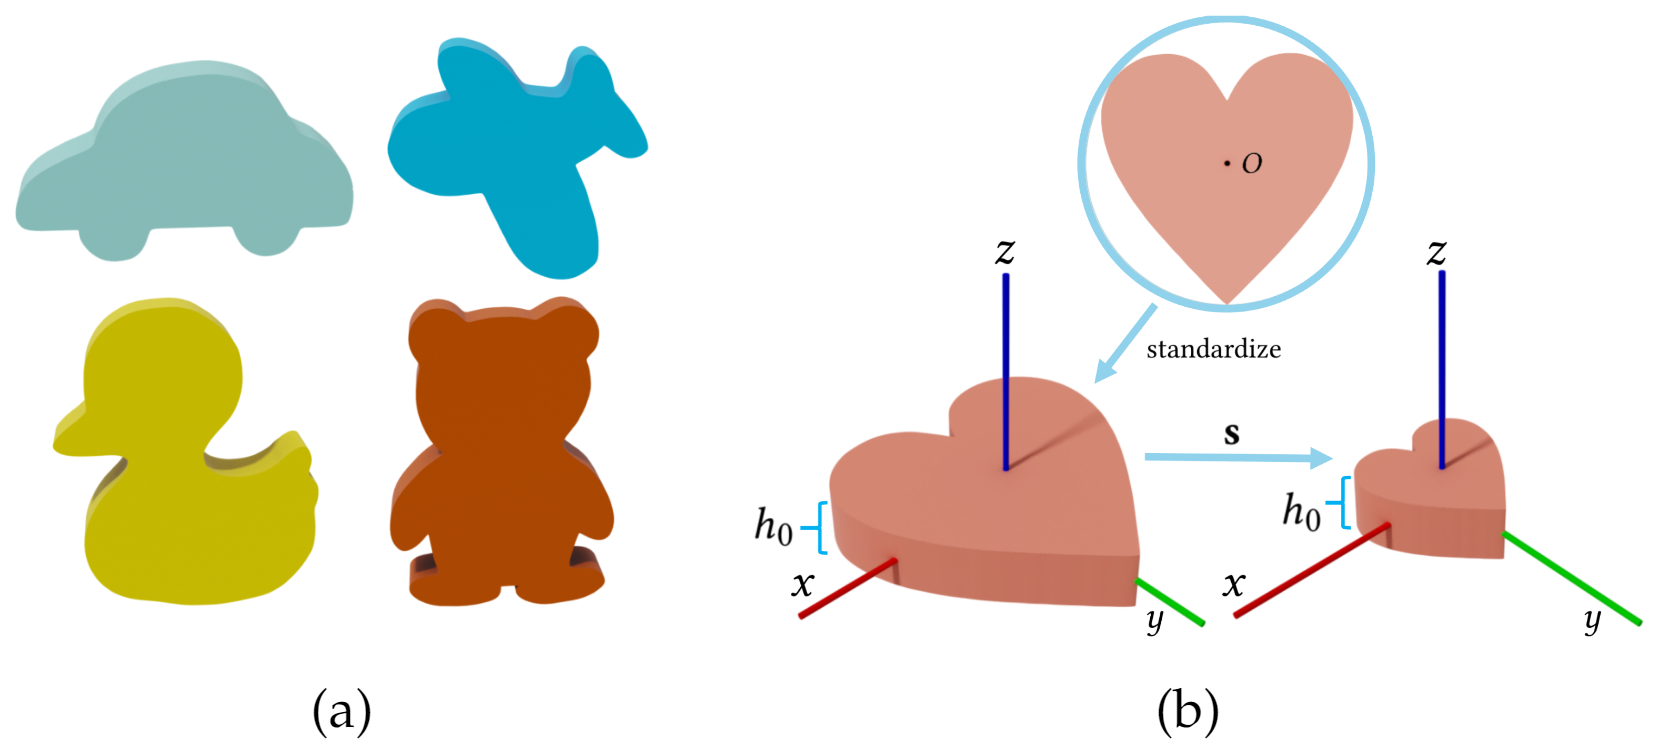
\includegraphics[width=1.0\linewidth]{./figures/custom-pattern}
    \caption{个性化图案模板构造示意图}
    \label{fig-custom}
\end{figure}
如图~\ref{fig-custom}所示,个性化图案模板的设计变量是 $\{\mathbf{c}_0, s_x, \mathbf{R}\}$。其中,模板的厚度不会随着缩放而改变,即$s_x=s_y$和$s_z=1$。

\subsubsection{雕刻设计} 
在薄壳上雕刻图案模板,是通过输入壳体与图案模板之间布尔运算的实现。得益于基于函数的表示,复杂的布尔运算可以简化为函数的最小值计算。图案模板的主要特征有位置、定向和尺寸等。具体的:
\paragraph{图案模板的位置。}
在薄壳结构上分配图案模板的位置是至关重要的,如图~\ref{fig-shellCarved} (b)所示,首先在薄壳结构的中心表面上利用Lloyd算法~\cite{levy2010p}计算一个受限的Voronoi图,然后将图案模板放置在Voronoi单元的质心处$\{\mathbf{c}_0^i=(x_0^i, y_0^i, z_0^i)\}_{i=1}^{N_p}$,$N_p$是图案模板的数量。Voronoi 镶嵌已广泛应用于壳体设计,并与设计的非规则图案模板兼容。本文提出的框架可以用于直接优化图案的位置,然而,优化变量和计算成本将急剧增加。因此,本文利用 Voronoi 图来简化算法的计算。未来将研究探索一种更高效、更优化的方法来确定图案的位置。
\begin{figure}[htbp]
    \centering
    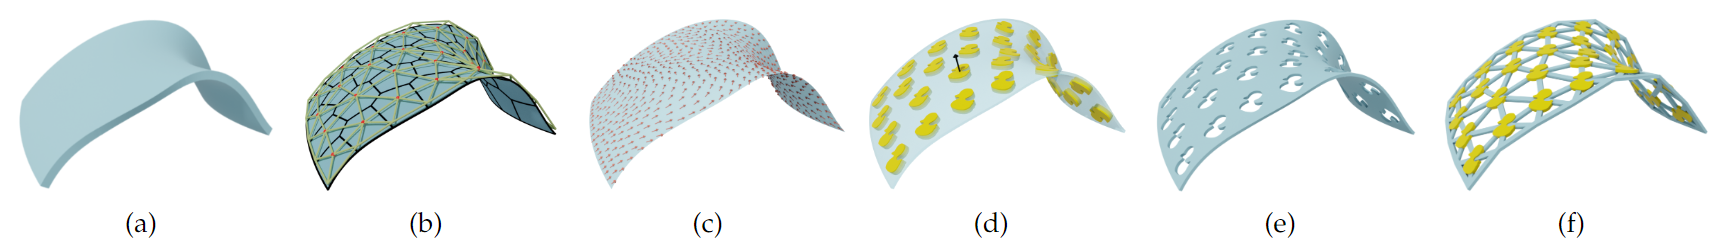
\includegraphics[width=1.0\linewidth]{./figures/algorithm-pipeline}
    \caption{薄板(对偶)雕刻算法流程示意图}
    \label{fig-shellCarved}
\end{figure}

\paragraph{图案模板的定向。}
图案的方向包括两个步骤:分别设置局部坐标系中 $z$ 轴方向和 $xy$ 平面上的旋转方向。
首先,通过方向矩阵 $\mathbf{R}_i^z$ 旋转图案,使局部坐标系的 $z$ 轴方向与中心面上相应 Voronoi 单元的法向量 $\{\mathbf{n}_c^i\}_{i=1}^{N_p}$ 对齐。
特别地,如果 $\mathbf{n}_c^i=\mathbf{z}_0$,其中 $\mathbf{z}_0=(0,0,1)^T$,则方向矩阵 $\mathbf{R}_i^z=\mathbf{I}_{3\times 3}$;否则,$\mathbf{R}_i^z$ 可以计算为
\begin{equation}
	\begin{split}
		& \mathbf{n}_z^i=\mathbf{n}_c^i,\\
		& \mathbf{n}_x^i=\frac{\mathbf{n}_x^i\times\mathbf{z}_0}{\|\mathbf{n}_x^i\times\mathbf{z}_0\|},\\ 
		&\mathbf{n}_y^i=\frac{\mathbf{n}_z^i\times\mathbf{n}_x^i}{\|\mathbf{n}_z^i\times\mathbf{n}_x^i\|},\\
		& \mathbf{R}^z_i=(\mathbf{n}_x^i, \mathbf{n}_y^i, \mathbf{n}_z^i)^T.
	\end{split}
\end{equation}
然后,根据旋转角度旋转图案模板,确定局部坐标系中 $xy$ 平面上模板的方向。因此,图案模板的方向可以通过旋转矩阵确定,如下所示:
\begin{equation}
    \mathbf{R}_i=\Lambda(\alpha_i)\mathbf{R}_i^z,
\end{equation}
其中, $\{\alpha_i\}_{i=1}^{N_p}$ 是可设计的旋转角度。
此外,本文提出的方法允许通过生成方向场~\cite{Directional}来确定旋转角度,如图~\ref{fig-shellCarved} (c) 所示,规则的方向场可以实现更美观的图案模板分布。

\paragraph{图案模板的尺寸。}
图案模板应限制在相应的 Voronoi 单元内,以避免相交。此外,相邻图案模板不应太近以保证可打印性和可用性。因此,算法将第 $i$ 个图案的最大尺寸长度设置为
\begin{equation}
	L_{\max}^i=e^i_b-\epsilon/2,
\end{equation}
其中,$e^i_b$是当前中心点与Voronoi单元边界之间的最小距离,$\epsilon$是最小打印精度。图案的最小尺寸长度可根据应用需求指定。在本文的实验中,默认设置第$i$个图案的最小尺寸长度$L_{\min}^i$为输入壳体厚度的一半。

\paragraph{薄壳雕刻操作。}
为了隐式设计薄壳结构,本文使用有向距离函数$\phi_{\mathrm{shell}}(\mathbf{r})$表示输入的壳体模型。在壳体上进行雕刻设计就是要移除壳体的部分区域,由于图案和输入壳体都用函数表示,复杂的布尔运算可以转化为以下简单计算:
\begin{equation}
	\Phi^{E}(\mathbf{r})=\min(\phi_{\mathrm{shell}}(\mathbf{r}), P_1(\mathbf{r}), P_2(\mathbf{r}),\cdots,P_{N_p}(\mathbf{r})),
\end{equation} 
其满足:
\begin{equation}
	\Phi(\mathbf{r})
	\begin{cases}
		>0, & \text{如果 $\mathbf{r}$ 在雕刻模型的内部},\\
		=0, & \text{如果 $\mathbf{r}$ 在雕刻模型的边界},\\
		<0, & \text{如果 $\mathbf{r}$ 在雕刻模型的外部}.
	\end{cases}
\end{equation}
雕刻后的壳体结构是函数$\Phi(\mathbf{r})$的零等值面,如图~\ref{fig-shellCarved}(e)所示。

\paragraph{薄壳对偶雕刻操作。}
与所提出的算法相容另一种薄壳结构设计方式是,将与壳体相交的图案模板部分保留为实体而不是挖空,我们称之为对偶雕刻设计。在本研究中,通过简单的函数修改实现对偶雕刻,所有保留的实体部分可表示为:
\begin{equation}
    \begin{split}
        &\phi_{\mathrm{retain}}=\max(\tilde{P}_1(\mathbf{r}), \tilde{P}_2(\mathbf{r}), \cdots, \tilde{P}_{N_p}(\mathbf{r})),\\
        &\tilde{P}_i(\mathbf{r})=\min(\phi_{\mathrm{shell}}(\mathbf{r}), -P_i(\mathbf{r})), \,\, i=1,2,\cdots, N_p.
    \end{split}
\end{equation}
为了将各个图案模板之间连接起来,算法使用Voronoi镶嵌的对偶Delaunay三角形的边构建一组桁架结构,如图~\ref{fig-shellCarved}(b)所示。对于开放曲面,还需要添加边来连接Delaunay三角形的边界点和Voronoi镶嵌的边界点。假设Delaunay三角形具有边集$\{e_i\}_{i=1}^{N_e}$,使用公式~(\ref{eq-ellipsoid})中描述的超椭球方程构建桁架结构:
\begin{equation}
    \begin{split}
        &\phi_{\mathrm{truss}} = \max(\tilde{E}_1(\mathbf{r}), \tilde{E}_2(\mathbf{r}), \cdots, \tilde{E}_{N_e}(\mathbf{r})),\\
        &\tilde{E}_i(\mathbf{r})=\min(\phi_{\mathrm{shell}},E_i(\mathbf{r})),\,\, i = 1, 2, \cdots, N_e,
    \end{split}
\end{equation}
其中,${E_i(\mathbf{r})}{i=1}^{N_e}$是一系列超椭球,将每条边的中点设置为相应超椭球的中心,边的方向决定了旋转矩阵$\mathbf{R}={R{ij}}_{3\times 3}$,$L_2$设置为边长的一半,$L_1$和$L_3$被释放以优化调整桁架结构的局部厚度。对于桁架的构建,设置$p=8$。在本文的实验中,$L_1$和$L_3$根据输入壳体在外部载荷下的应变能分布来分配。
最终,对偶雕刻可以隐式表示为
\begin{equation}
	\Phi^{DE}(\mathbf{r})=\max(\phi_{\mathrm{retain}}, \phi_{\mathrm{truss}}).
\end{equation}
类似地,提取函数$\Phi^{DE}(\mathbf{r})$的零等值面以获得对偶雕刻壳体结构,如图~\ref{fig-shellCarved}(f)所示。